\documentclass[11pt,a4paper]{article}
\usepackage[margin=22mm]{geometry}
\usepackage{fontspec}
\setmainfont{Arial}
\setsansfont{Arial}
\usepackage{amsmath,amssymb,graphicx,booktabs,tabularx,longtable,float,hyperref,tikz,fancyhdr}
\usetikzlibrary{positioning,arrows.meta}
\hypersetup{colorlinks=true,linkcolor=blue,urlcolor=blue}
\pagestyle{fancy}\fancyhf{}
\fancyhead[L]{ME5411 Robot Vision and AI}
\fancyhead[R]{Group 33 -- Draft}
\fancyfoot[C]{\thepage}
\setlength{\headheight}{14pt}
\setlength{\parindent}{0pt}
\setlength{\parskip}{6pt}
\linespread{1.0}
\emergencystretch=3em
\newcommand{\review}[1]{\begin{quote}\textbf{Group review required.} #1\end{quote}}
\newcommand{\fig}[3]{\begin{figure}[H]\centering\includegraphics[width=\linewidth,height=#2\textheight,keepaspectratio]{figures/#1.png}\caption{#3}\end{figure}}
\newcommand{\topic}[1]{\clearpage\section{#1}}
\begin{document}
\hypersetup{pageanchor=false}
\begin{titlepage}\centering
\vspace*{18mm}
{\Large National University of Singapore\par}
\vspace{8mm}{\Large ME5411 Robot Vision and AI\par}
\vspace{16mm}{\LARGE Character Recognition on a Microchip\par}
\vspace{6mm}{\large Image Processing, CNN and HOG--SVM\par}
\vspace{14mm}{\Large Group 33\par}
\vspace{8mm}
\begin{tabular}{ll}\toprule Member name & Student number\\\midrule
{[Full name]} & {[Student number]}\\
{[Full name]} & {[Student number]}\\
{[Full name]} & {[Student number]}\\\bottomrule\end{tabular}
\vfill
\textbf{Report draft for group review}\par
Methods and recorded experimental evidence, with discussion prompts.\par
Prepared 17 November 2026\par
Submission deadline 20 November 2026, 23:59 Singapore time.
\end{titlepage}
\hypersetup{pageanchor=true}
\begingroup
\setlength{\parskip}{0pt}
\makeatletter
\renewcommand{\l@section}{\@dottedtocline{1}{0em}{2.5em}}
\makeatother
\tableofcontents
\endgroup
\topic{Draft status and introduction}
The project investigates image processing and character classification for a microchip label. Tasks 1--6 cover contrast adjustment, smoothing, cropping, binarization, boundary extraction and connected-component segmentation. Task 7 compares a convolutional neural network (CNN) with a histogram-of-oriented-gradients (HOG) and support-vector-machine (SVM) classifier.

The supplied bitmap is \path{task7/dataset_2026/Test_Image_2026.bmp}. The user identified it as the assignment's \texttt{charact2.bmp}. It has 990 columns and 367 rows. The requested line is \texttt{HD44780A00}. The supplied training vocabulary contains the seven classes 0, 4, 7, 8, A, D and H.

This draft describes the current repository and transcribes its saved results. Task 1--6 illustrations are exported from saved outputs in \path{task1-6/tasks.ipynb}. Task 7 figures and measurements come from \path{task7/results/}.

The assignment permits LLM use for language editing and requires ideas, analysis and reasoning to originate from the group. This draft was assembled with AI assistance. The group must verify the technical account, supply its own interpretation in the marked discussion areas, and check permitted use before submission. Statements identified as notebook observations reproduce existing project observations.

The group number follows the notebook's Group 33 heading. Member details remain to be completed. The document uses 11-point Arial and single spacing. The assignment specifies a maximum of 50 pages and describes 30--40 pages as typical. This draft prioritizes the available evidence and still requires the group's discussion.
\review{Confirm member details, the course coverage of the selected SVM method, and the final report wording.}
\topic{Implementation map and overall flow}
\begin{tabularx}{\linewidth}{@{}lX@{}}\toprule
Requirement & Current implementation\\\midrule
Tasks 1--4 & \path{task1-6/tasks.ipynb}, functions in \texttt{preprocessing.py}\\
Task 5 & \texttt{character\_outlines}, inner morphological boundary\\
Task 6 & \texttt{prepare\_character\_binary}, \texttt{connected\_components}\\
Task 7-1 & \texttt{task7/models.py}, \texttt{task7/train.py}\\
Task 7-2 & HOG and linear squared-hinge SVM in the same modules\\
Task 7-3 & Recorded metrics, figures and \texttt{summarize\_results.py}\\\bottomrule
\end{tabularx}
\begin{center}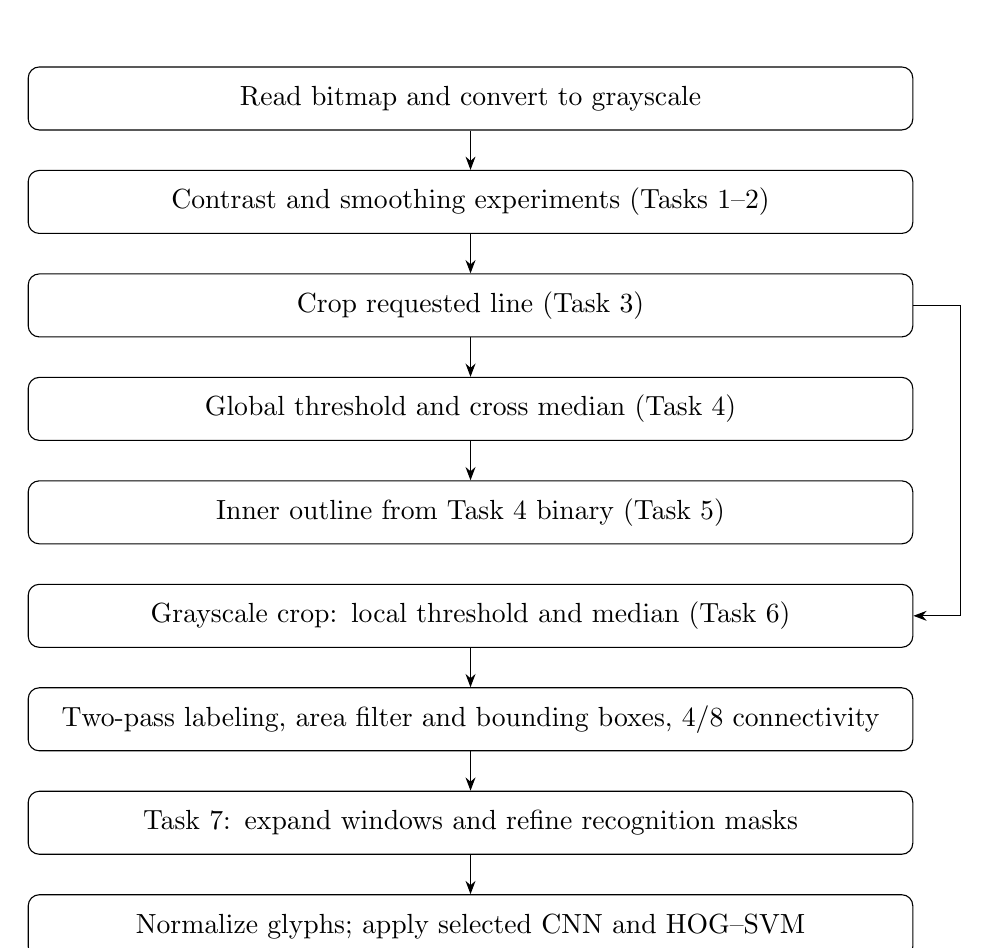
\begin{tikzpicture}[node distance=5mm,every node/.style={draw,rounded corners,align=center,text width=11cm,minimum height=8mm},>=Stealth]
\node (a) {Read bitmap and convert to grayscale};
\node[below=of a] (b) {Contrast and smoothing experiments (Tasks 1--2)};
\node[below=of b] (c) {Crop requested line (Task 3)};
\node[below=of c] (d) {Global threshold and cross median (Task 4)};
\node[below=of d] (e) {Inner outline from Task 4 binary (Task 5)};
\node[below=of e] (f) {Grayscale crop: local threshold and median (Task 6)};
\node[below=of f] (g) {Two-pass labeling, area filter and bounding boxes, 4/8 connectivity};
\node[below=of g] (h) {Task 7: expand windows and refine recognition masks};
\node[below=of h] (i) {Normalize glyphs; apply selected CNN and HOG--SVM};
\foreach \x/\y in {a/b,b/c,c/d,d/e,f/g,g/h,h/i}\draw[->](\x)--(\y);
\draw[->] (c.east) -- ++(0.6,0) |- (f.east);
\end{tikzpicture}\end{center}
Task 6 starts from the Task 3 grayscale crop. Its binary preparation is distinct from the Task 4 input used for outlines. Task 7 bundles the relevant Task 6 functions in \texttt{segmentation.py} and adds bounded mask refinement in \texttt{chip\_processing.py}. Its dataset and selected models are included for independent use.
\topic{Task 1 -- original image and contrast methods}
\fig{original}{.30}{Saved original bitmap display and intensity histogram.}
The notebook converts the OpenCV BGR image to grayscale. It compares linear contrast stretching with bounds 70 and 170, piecewise stretching through $(70,20)$ and $(170,240)$, thresholds 100 and 110, global histogram equalization, and CLAHE with clip limit 1.2 and a $4\times4$ tile grid.

Linear stretching maps the selected interval to the display range and clips intensities outside it. The notebook's piecewise transform provides a different mapping for the lower, middle and upper input ranges. Thresholding returns 255 for values at or above the threshold and zero otherwise. Histogram equalization is delegated to OpenCV, as is CLAHE.

The saved notebook observations state that thresholding increases visible foreground/background separation while also exposing background texture. Raising the threshold from 100 to 110 reduces visible background responses on this image. The notebook describes contrast stretching as a visual compromise and notes that global equalization amplifies background variation. These are qualitative observations for this bitmap.
\review{Explain which contrast display the group prefers, identify the relevant visible regions, and distinguish appearance from downstream segmentation performance.}
\topic{Task 1 -- intermediate contrast results}
\fig{contrast}{.83}{Saved comparison of seven contrast settings with their corresponding histograms. Settings and labels reproduce the notebook output.}
\topic{Task 2 -- averaging filter}
For an odd window width $k$, the manually implemented filter computes
\[
I_k(x,y)=\operatorname{round}\left(\frac{1}{k^2}\sum_{u=-r}^{r}\sum_{v=-r}^{r}I(x+u,y+v)\right),\qquad r=(k-1)/2.
\]
The handwritten path pads using edge replication, computes a mean at each pixel, rounds and clips to the 8-bit range. The optional OpenCV path uses constant padding. The notebook's main averaging comparison uses the handwritten path. Boundary behavior therefore depends on the selected implementation.

The investigated sizes are $1,3,5,7,9,11,13,15$. The required $5\times5$ case is included. The $1\times1$ result provides the unchanged grayscale reference.
\fig{average}{.50}{Saved averaging-filter comparison, including the required $5\times5$ result.}
The notebook records a visual preference for $7\times7$ as a balance between smoothing and sharpness. It does not measure noise statistics or identify the noise distribution from ground truth.
\topic{Task 2 -- square and cross median comparisons}
The square median uses all $k^2$ window pixels. The cross median uses the central row and column, with the center counted once, giving $2k-1$ samples. Both compare odd support widths from 1 to 15. The square results use OpenCV; the cross is implemented by selecting pixels with a Boolean mask.
\fig{square_median}{.31}{Saved square-median comparison.}
\fig{cross_median}{.31}{Saved cross-median comparison.}
\review{Use visible stroke and background changes to discuss the effect of support shape and size. The notebook's description of ring-like texture is a visual observation, and does not establish a noise model.}
\topic{Task 2 -- combined processing experiments}
The notebook additionally applies averaging to the $13\times13$ cross-median image. It displays a $5\times5$ average followed by contrast stretching from 100 to 150, and the same filtered image followed by threshold 110. A separate trial thresholds first and then applies a $15\times15$ cross median.
\fig{combined_stretch}{.22}{Cross median 13, average 5 and contrast stretch 100--150.}
\fig{combined_threshold}{.22}{Cross median 13, average 5 and threshold 110.}
\fig{threshold_median}{.22}{Threshold 110 followed by cross median 15.}
\review{Describe the changes observed when the processing order changes. Explain the group's eventual choice using these results.}
\topic{Tasks 3--4 -- crop and binary conversion}
The ROI is recorded as $(x,y,w,h)=(36,202,912,136)$ in zero-based pixel coordinates. NumPy extracts rows \texttt{202:338} and columns \texttt{36:948}. This manual ROI contains the requested second line.
\fig{crop}{.19}{Saved grayscale ROI and histogram.}
Task 4 thresholds this grayscale crop at 110 and applies cross-median filters of width 23 and 13. Foreground pixels have value 255. The width-23 result, \texttt{median\_sub}, is passed to Task 5.
\fig{task4_binary}{.19}{Saved Task 4 grayscale and threshold-110 binary display.}
\fig{task4_median}{.19}{Saved Task 4 cross-median comparison, width 23 on the first row and width 13 on the second row.}
\topic{Task 5 -- morphological character outlines}
Let $B$ denote the foreground set and let $S$ be a $3\times3$ square structuring element. The inner outline is
\[
\partial B=B\setminus(B\ominus S).
\]
The implementation interprets every nonzero input as foreground, pads the foreground with zeros, and retains a pixel in the eroded image only if its complete $3\times3$ neighborhood is foreground. The output is 255 at foreground pixels removed by erosion. This includes boundaries surrounding holes, where present in the input.
\fig{task5_outline}{.37}{Task 4 width-23 cross-median binary and its inner outline, as saved in the notebook.}
The outline inherits the topology and residual foreground of its input. Finding a boundary does not identify a character class. Its role here is to visualize the edge of the filtered foreground.
\review{Inspect which holes and stroke edges remain visible. Explain whether the Task 4 filter preserves the details the group considers relevant.}
\topic{Task 6 -- binary preparation for segmentation}
Task 6 returns to the grayscale ROI. The stages are a $3\times3$ average, a $31\times31$ local-mean estimate, local thresholding with offset 4, and a $5\times5$ square median. In the implementation,
\[
B(x,y)=255\,\mathbf{1}\{I_s(x,y)\geq\mu_{31}(x,y)+4\}.
\]
The bright foreground is selected relative to the surrounding mean. The parameters are fixed for this chip image and are shared by both connectivity experiments.
\fig{task6_binary}{.45}{Saved grayscale crop, smoothed crop and locally thresholded median-filtered binary.}
Course references have been checked against the supplied lecture export. Chapter 3, Image Preprocessing Part 2, p. 26 describes averaging and pp. 31--34 describe median filtering. Chapter 4, Segmentation Part 1, p. 16 defines local thresholding using neighborhood properties, including average gray level. Its pp. 31--34 describe connectivity and two-pass labeling, and pp. 39--40 describe region area.
\review{Explain the choice of local intensity comparison and comment on any residual attached background visible in the resulting glyphs.}
\topic{Task 6 -- two-pass connected components}
For 4-connectivity, the first raster scan examines the already visited left and upper neighbors. For 8-connectivity it also examines upper-left and upper-right. A foreground pixel receives a new label if no labeled neighbor exists. Otherwise it receives a neighboring label, and equivalences are recorded when different neighboring labels meet.

The second pass resolves the equivalences and accumulates area and bounding coordinates for each region. The component list retains regions with at least 500 pixels, then orders them left to right. The label image still represents all foreground regions. Each retained character box is derived from one component.
\begin{center}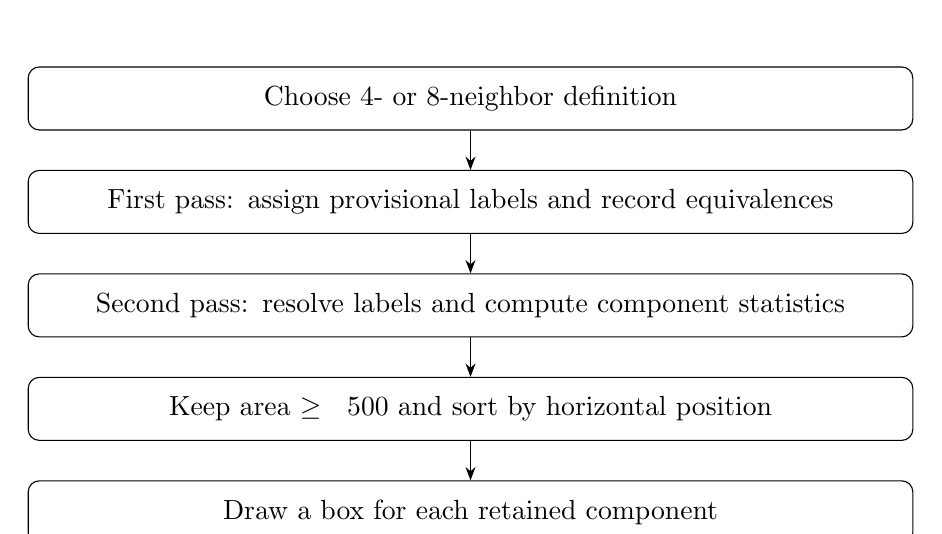
\begin{tikzpicture}[node distance=5mm,every node/.style={draw,rounded corners,align=center,text width=11cm,minimum height=8mm},>=Stealth]
\node(a){Choose 4- or 8-neighbor definition};
\node[below=of a](b){First pass: assign provisional labels and record equivalences};
\node[below=of b](c){Second pass: resolve labels and compute component statistics};
\node[below=of c](d){Keep area $\geq500$ and sort by horizontal position};
\node[below=of d](e){Draw a box for each retained component};
\foreach \x/\y in {a/b,b/c,c/d,d/e}\draw[->](\x)--(\y);
\end{tikzpicture}\end{center}
\begin{center}\begin{tabular}{lrr}\toprule Setting & All regions & Retained regions\\\midrule
4-connectivity & 138 & 10\\8-connectivity & 138 & 10\\\bottomrule\end{tabular}\end{center}
A saved diagonal sanity check uses a $3\times3$ identity pattern. It yields three components under 4-connectivity and one under 8-connectivity. Equal counts on the chip are therefore compatible with distinct neighborhood definitions.
\topic{Task 6 -- bounding boxes and character labels}
\fig{task6_boxes}{.39}{Saved 4- and 8-connectivity results. Box numbers indicate left-to-right segmentation positions.}
The saved component records agree across both connectivity settings. Coordinates below are relative to the ROI.
\begin{center}\begin{tabular}{rrrrrr}\toprule Position & $x$ & $y$ & Width & Height & Area\\\midrule
1 & 24 & 11 & 84 & 121 & 3932 \\
2 & 116 & 2 & 87 & 134 & 4302 \\
3 & 206 & 10 & 82 & 126 & 3517 \\
4 & 296 & 12 & 87 & 116 & 3364 \\
5 & 387 & 0 & 90 & 128 & 2756 \\
6 & 469 & 11 & 88 & 117 & 4467 \\
7 & 559 & 7 & 85 & 124 & 3973 \\
8 & 646 & 10 & 91 & 117 & 3290 \\
9 & 731 & 6 & 86 & 122 & 4086 \\
10 & 824 & 5 & 82 & 124 & 4082 \\
\bottomrule\end{tabular}\end{center}
The original image position of a box is obtained by adding 36 to its horizontal coordinate and 202 to its vertical coordinate. Component labels stored internally differ from the positional numbers displayed above.
\review{Assess the quality of the retained character masks and the sensitivity of the 500-pixel cutoff. The recorded experiment verifies this image and these settings.}

\topic{Task 7 -- dataset and evaluation protocol}
The dataset contains 7,112 grayscale $128\times128$ character images, with 1,016 images in each of seven classes. The class order is 0, 4, 7, 8, A, D and H. Class images are loaded from their subfolders. The chip bitmap supplies the character-recognition application.
\begin{center}\begin{tabular}{lrrrr}\toprule
Class & Inner train & Validation & Development & Test\\\midrule
0 & 610 & 152 & 762 & 254\\
4 & 610 & 152 & 762 & 254\\
7 & 610 & 152 & 762 & 254\\
8 & 610 & 152 & 762 & 254\\
A & 610 & 152 & 762 & 254\\
D & 610 & 152 & 762 & 254\\
H & 610 & 152 & 762 & 254\\\midrule
Total & 4270 & 1064 & 5334 & 1778\\\bottomrule
\end{tabular}\end{center}
Development comprises the required 75\% and test comprises 25\%. Development is internally divided into training and validation portions. Following configuration selection, each selected model is initialized again and fitted on all 5,334 development images.

Direct comparison of decoded grayscale dimensions and pixel bytes identifies 5,850 unique arrays and 651 duplicate groups, with 1,262 additional copies. Whole exact-duplicate groups stay within a single partition. The manifest records zero cross-partition exact-duplicate groups. The seed for partitioning and the main configuration search is 5411. The data loader reads the image paths and partition assignments from the manifest. Related fonts and near-duplicate images can span partitions because font-family identifiers are unavailable.

The chip bitmap supplies feedback for image-processing development. Classifier fitting uses the class-image dataset. The shared test partition and chip example had been observed during project development. The reported measurements describe the saved split and the supplied chip example.

\topic{Task 7 -- shared parameter search and selection}
The implementation combines architecture, preprocessing, regularization, feature and optimization comparisons within one experiment registry. Candidate values are declared in \path{task7/search_space.json}. The registry contains 95 trial records, all using seed 5411. One main-seed SVM trial encounters a nonfinite loss and is recorded as failed.

For each successful trial, the validation score selects the earliest epoch attaining its highest accuracy. Final selection compares configurations using their validation accuracy at seed 5411, with ties resolved by fewer learned parameters and then an earlier best epoch. The selected trial's best epoch supplies the development-refit budget. The selected configuration is frozen before its final refit and test evaluation.

The search proceeds through groups. Later groups can start from the strongest recorded main-seed configuration and vary specified factors. The appendix lists every record with its settings, seed, selected epoch and validation score. The table below records the selected configurations.
\begin{center}\begin{tabular}{lrrr}
\toprule
Model & Seed & Validation accuracy & Refit epochs \\\midrule
CNN & 5411 & 99.91\% & 9 \\
SVM & 5411 & 99.72\% & 9 \\
\bottomrule\end{tabular}\end{center}

The selected CNN has a 32-unit hidden layer and is refitted for nine epochs. The selected SVM uses Adam at learning rate 0.03 and is refitted for nine epochs. The final checkpoint class order and configuration are saved with its weights.
\review{Explain the group's reasons for the investigated parameter ranges and the validation-based selection procedure. Use the complete records when interpreting small score differences.}

\topic{Task 7 -- input normalization}
All classifier inputs are $32\times32$ float32 arrays in $[0,1]$, with bright character foreground. The three investigated modes use bilinear interpolation.
\begin{itemize}
\item \texttt{resize} inverts the grayscale image and resizes the complete image.
\item \texttt{pad} crops around inverted intensity values above 51, centers the crop on a square canvas, adds a per-side margin of 12\% of the longer side with a minimum of two pixels, and resizes.
\item \texttt{stretch} uses the same intensity-based crop and resizes the cropped rectangle directly to $32\times32$.
\end{itemize}
\fig{preprocessing_examples}{.55}{Training-image examples for complete-image resize, square padding and cropped stretch. Each row corresponds to one class.}
Both selected classifiers use \texttt{stretch}. Chip glyphs are first represented as dark foreground on white backgrounds, then passed through the normalization recorded in their checkpoints.

\topic{Subtask 7-1 -- selected CNN and architecture comparison}
\begin{center}\begin{tabularx}{\linewidth}{@{}lXl@{}}\toprule
Stage & Operation & Output shape\\\midrule
Input & Normalized grayscale glyph & $1\times32\times32$\\
1 & Conv $3\times3$, 16 channels, ReLU, max pool 2 & $16\times16\times16$\\
2 & Conv $3\times3$, 32 channels, ReLU, max pool 2 & $32\times8\times8$\\
Pooling & Adaptive average pool to $8\times8$ & $32\times8\times8$\\
Dense & Flatten, linear 2048 to 32, ReLU & 32\\
Output & Linear 32 to 7 logits & 7\\\bottomrule
\end{tabularx}\end{center}
The selected CNN has 70,599 learned parameters. All convolutions use padding one. Cross-entropy is minimized with Adam, learning rate 0.003 and batch size 32. The selected dropout and weight-decay values are both zero. Training uses CPU execution with four threads.

The architecture investigation compares convolution depths two and three, average-pooling widths four and eight, and the four combinations of dropout 0 or 0.25 and weight decay 0 or $10^{-4}$. The table holds preprocessing at \texttt{pad}, hidden width at 64, Adam learning rate at 0.003 and batch size at 128.
\begin{center}\begin{tabular}{rrrrrr}
\toprule
Depth & Pool & FC input & Dropout & Weight decay & Validation \\\midrule
2 & 4 & 512 & 0 & 0 & 99.15\% \\
2 & 4 & 512 & 0 & 0.0001 & 98.97\% \\
2 & 4 & 512 & 0.25 & 0 & 98.97\% \\
2 & 4 & 512 & 0.25 & 0.0001 & 98.97\% \\
2 & 8 & 2048 & 0 & 0 & 99.34\% \\
2 & 8 & 2048 & 0 & 0.0001 & 99.25\% \\
2 & 8 & 2048 & 0.25 & 0 & 99.25\% \\
2 & 8 & 2048 & 0.25 & 0.0001 & 99.06\% \\
3 & 4 & 1024 & 0 & 0 & 99.25\% \\
3 & 4 & 1024 & 0 & 0.0001 & 99.25\% \\
3 & 4 & 1024 & 0.25 & 0 & 99.25\% \\
3 & 4 & 1024 & 0.25 & 0.0001 & 99.25\% \\
3 & 8 & 4096 & 0 & 0 & 99.34\% \\
3 & 8 & 4096 & 0 & 0.0001 & 99.53\% \\
3 & 8 & 4096 & 0.25 & 0 & 99.34\% \\
3 & 8 & 4096 & 0.25 & 0.0001 & 99.25\% \\
\bottomrule\end{tabular}\end{center}

The fully connected input depends on both the final convolutional channel count and the pooling grid. The investigated input widths are 512, 1024, 2048 and 4096.

\topic{Subtask 7-1 -- hidden width, regularization and preprocessing}
The hidden-width comparison uses depth two, an $8\times8$ pooling grid, \texttt{stretch}, Adam learning rate 0.003 and batch size 32. Dropout and weight decay are zero.
\begin{center}\begin{tabular}{rrrr}
\toprule
Hidden width & Parameters & Best epoch & Validation \\\midrule
32 & 70599 & 9 & 99.91\% \\
64 & 136391 & 7 & 99.72\% \\
128 & 267975 & 11 & 99.91\% \\
\bottomrule\end{tabular}\end{center}

Hidden widths 32 and 128 attain the same highest validation accuracy. The tie is resolved by the smaller parameter count, selecting hidden width 32 and its best epoch, nine.

Regularization is also compared around the 32-unit hidden-layer configuration, with the other settings fixed.
\begin{center}\begin{tabular}{rrrr}
\toprule
Dropout & Weight decay & Best epoch & Validation \\\midrule
0 & 0 & 9 & 99.91\% \\
0 & 0.0001 & 12 & 99.72\% \\
0.25 & 0 & 15 & 99.81\% \\
0.25 & 0.0001 & 14 & 99.81\% \\
\bottomrule\end{tabular}\end{center}

The final selected configuration uses zero dropout and zero weight decay. The records describe the investigated dataset, training budget and validation partition.

The preprocessing group compares \texttt{resize}, \texttt{pad} and \texttt{stretch}, and a separate batch-size group compares 32 and 128. Their complete settings and scores appear in the appendix. Changing these factors also changes the normalized geometry or the sequence of parameter updates.
\begin{center}\begin{tabular}{lrr}
\toprule
Mode & Best epoch & Validation \\\midrule
resize & 15 & 99.53\% \\
pad & 11 & 99.25\% \\
stretch & 9 & 99.91\% \\
\bottomrule\end{tabular}\end{center}

\review{Interpret the parameter-count and validation measurements for the investigated CNNs. Explain the group's choice of model capacity and regularization using the controlled comparisons at seed 5411.}

\topic{Subtask 7-1 -- optimization and learning histories}
Adam, AdamW and momentum SGD are compared around the selected depth, pooling, hidden width and preprocessing. AdamW uses weight decay $10^{-4}$. SGD uses momentum 0.9. Each optimizer is evaluated at the learning rates shown below.
\begin{center}\begin{tabular}{lrrrr}
\toprule
Optimizer & Learning rate & Best epoch & Fit (s) & Validation \\\midrule
ADAM & 0.001 & 18 & 19.095 & 99.53\% \\
ADAM & 0.003 & 9 & 18.500 & 99.91\% \\
ADAMW & 0.001 & 18 & 19.102 & 99.53\% \\
ADAMW & 0.003 & 7 & 18.728 & 99.81\% \\
SGD & 0.01 & 19 & 17.774 & 99.62\% \\
SGD & 0.03 & 11 & 17.656 & 99.72\% \\
SGD & 0.1 & 9 & 17.164 & 98.59\% \\
\bottomrule\end{tabular}\end{center}

\fig{cnn_optimizer_comparison}{.30}{Recorded CNN validation accuracy by optimizer and learning rate. The complete configurations accompany the experiment records.}
\fig{cnn_learning_curves}{.30}{Training cross-entropy and validation accuracy for the selected CNN configuration at seed 5411.}

\topic{Subtask 7-2 -- handwritten HOG and margin classifier}
HOG is implemented using NumPy. Image gradients yield magnitude and unsigned orientation. Each cell accumulates nine bins over $[0,\pi)$ with interpolation between neighboring orientation bins. Overlapping $2\times2$-cell blocks undergo L2 normalization, clipping at 0.2 and renormalization. Pixel votes are assigned to their spatial cell.

For a $32\times32$ glyph, $8\times8$-pixel cells yield $3\times3$ blocks and $3\times3\times4\times9=324$ features. The $4\times4$-pixel cells yield $7\times7\times4\times9=1764$ features. Flattened pixels supply a 1,024-dimensional comparison.

Seven linear one-vs-rest functions produce scores $s_c=w_c^T\phi(x)+b_c$. The margin objective is
\[
L=\frac12\sum_c\|w_c\|^2+
\frac{C}{N}\sum_i\sum_c\max(0,1-y_{ic}s_c(x_i))^p,
\]
where $y_{ic}=+1$ for the correct class and $-1$ for the remaining classes. The investigated exponents are $p=1$ for hinge loss and $p=2$ for squared-hinge loss. Biases are unregularized. The largest score determines the predicted class.

The selected model uses 1,764-dimensional HOG, squared-hinge loss, $C=100$, \texttt{stretch}, Adam learning rate 0.03 and batch size 128. It has 12,355 learned parameters and is refitted on development data for nine epochs.
\review{Explain the group's choice of a linear margin classifier and the role of orientation histograms in representing character shapes. Relate the margin objective to the relevant course material.}

\topic{Subtask 7-2 -- features, preprocessing and margin parameters}
The feature comparison fixes squared-hinge loss, $C=10$, Adam learning rate 0.01 and batch size 128. HOG uses eight-pixel cells in this table.
\begin{center}\begin{tabular}{llrr}
\toprule
Mode & Features & Best epoch & Validation \\\midrule
resize & PIXELS & 7 & 95.86\% \\
pad & PIXELS & 7 & 96.43\% \\
stretch & PIXELS & 12 & 98.21\% \\
resize & HOG & 11 & 95.96\% \\
pad & HOG & 20 & 96.62\% \\
stretch & HOG & 18 & 97.65\% \\
\bottomrule\end{tabular}\end{center}

The larger margin-parameter group crosses three preprocessing modes, two HOG cell widths, two loss definitions and four $C$ values. All 48 configurations appear in the appendix. The subset below fixes \texttt{stretch}, four-pixel HOG cells, Adam learning rate 0.01 and batch size 128.
\begin{center}\begin{tabular}{lrrr}
\toprule
Margin loss & $C$ & Best epoch & Validation \\\midrule
hinge & 0.1 & 28 & 92.39\% \\
hinge & 1 & 1 & 96.62\% \\
hinge & 10 & 9 & 98.12\% \\
hinge & 100 & 9 & 99.15\% \\
squared\_hinge & 0.1 & 1 & 95.30\% \\
squared\_hinge & 1 & 4 & 97.37\% \\
squared\_hinge & 10 & 20 & 98.97\% \\
squared\_hinge & 100 & 29 & 99.53\% \\
\bottomrule\end{tabular}\end{center}

These measurements provide comparisons within a fixed feature representation and training procedure. The learning rate is subsequently investigated in the optimizer group.

\topic{Subtask 7-2 -- optimization comparison}
The optimizer group fixes \texttt{stretch}, four-pixel HOG cells, squared-hinge loss and $C=100$. Adam and momentum SGD use minibatches of 128. LBFGS uses the full inner-training partition, with up to ten quasi-Newton iterations and a strong-Wolfe line search per recorded outer epoch. Its outer-epoch budget is fifteen.
\begin{center}\begin{tabular}{lrrrr}
\toprule
Optimizer & Learning rate & Best epoch & Fit (s) & Validation \\\midrule
ADAM & 0.003 & 13 & 0.982 & 99.44\% \\
ADAM & 0.01 & 29 & 0.913 & 99.53\% \\
ADAM & 0.03 & 9 & 0.964 & 99.72\% \\
SGD & 1e-05 & 27 & 0.850 & 98.68\% \\
SGD & 0.0001 & 30 & 0.853 & 99.44\% \\
SGD & 0.001 & 9 & 0.853 & 99.53\% \\
SGD & 0.01 & -- & -- & Failed \\
LBFGS & 1 & 3 & 1.724 & 99.44\% \\
\bottomrule\end{tabular}\end{center}

\fig{svm_optimizer_comparison}{.40}{Recorded SVM validation accuracy by optimizer and learning rate. The SGD trial at learning rate 0.01 is recorded as numerically failed.}
Epochs have optimizer-specific computational meaning. Fitting times accompany the score records. The selected SVM configuration maximizes validation accuracy at seed 5411.

\topic{Subtask 7-3 -- test effectiveness}
Accuracy is the fraction of correct test labels. Precision and recall are computed per class, and macro F1 averages the seven class F1 scores. Both selected classifiers are evaluated on the same 1,778 test images.
\begin{center}\begin{tabular}{llrrr}
\toprule
Model & Correct / total & Errors & Accuracy & Macro F1 \\\midrule
CNN & 1773 / 1778 & 5 & 99.72\% & 0.99719 \\
SVM & 1766 / 1778 & 12 & 99.33\% & 0.99324 \\
\bottomrule\end{tabular}\end{center}

The selected CNN has seven fewer test errors, corresponding to approximately 0.39 percentage points on this partition. Each selected method is refitted on development data at seed 5411 for its selected nine-epoch budget.
\begin{center}\begin{tabular}{lrrrr}
\toprule
Class & CNN precision & CNN recall & SVM precision & SVM recall \\\midrule
0 & 1.0000 & 0.9961 & 0.9883 & 0.9961 \\
4 & 1.0000 & 0.9961 & 0.9961 & 1.0000 \\
7 & 1.0000 & 0.9961 & 0.9922 & 1.0000 \\
8 & 1.0000 & 1.0000 & 1.0000 & 1.0000 \\
A & 0.9883 & 1.0000 & 0.9807 & 1.0000 \\
D & 0.9922 & 1.0000 & 0.9960 & 0.9843 \\
H & 1.0000 & 0.9921 & 1.0000 & 0.9724 \\
\bottomrule\end{tabular}\end{center}

CNN makes two H-to-A errors. SVM makes seven H-class errors, consisting of one H-to-4, two H-to-7 and four H-to-A errors. These counts are obtained from the saved test confusion matrices.
\review{Discuss the observed class confusions and the eight-error difference using the group's interpretation of the features and trained models. Address the evaluation partition and the range of supported classes.}

\topic{Subtask 7-3 -- test confusion matrices}
\fig{cnn_confusion}{.39}{Selected CNN confusion matrix. Rows represent true classes and columns represent predicted classes.}
\fig{svm_confusion}{.39}{Selected HOG--SVM confusion matrix on the same test images.}

\topic{Subtask 7-3 -- efficiency}
\begin{center}\begin{tabular}{lrr}
\toprule
Measurement & CNN & SVM \\\midrule
Learned parameters & 70599 & 12355 \\
Checkpoint bytes & 286569 & 51637 \\
Development refit (s) & 8.186 & 0.267 \\
Model time (ms/image) & 0.07695 & 0.00105 \\
HOG and model (ms/image) & -- & 0.55789 \\
\bottomrule\end{tabular}\end{center}

Model inference timing uses a four-thread CPU, one warm-up pass and the median of five full-test passes. File decoding, chip segmentation and image normalization are outside the timed interval. CNN model timing includes its learned feature extraction. SVM also has a feature-plus-model measurement covering handwritten HOG extraction from normalized arrays.

The refit measurement covers fitting the selected configuration on all development images. The trial registry separately records the preceding search fits and their histories. Checkpoint byte counts include serialization metadata.

The selected CNN records model inference of approximately 0.07695 ms per image. HOG extraction plus the selected SVM records approximately 0.55789 ms per image. The linear SVM score computation accounts for approximately 0.00105 ms per image within that pipeline. These measurements characterize this implementation and recorded runtime.
\review{Compare effectiveness, parameter count, fitting time, model inference and feature extraction for the intended application. Specify the timing scope used in each comparison.}

\topic{Chip recognition -- Task 6 masks and further image processing}
The saved CNN and SVM classifiers are applied to two character-input cases. Both use the recorded checkpoint-specific $32\times32$ normalization and the same classifier weights. Each extraction method is evaluated under 4-connectivity and 8-connectivity.

\textbf{Case 1. Task 6 binary character masks.} The reviewed Task 6 procedure uses a $3\times3$ mean, a $31\times31$ local mean with offset 4, and a $5\times5$ binary median. Connected-component labeling retains regions with area at least 500 and orders them from left to right. Each retained component directly supplies its binary character mask to the classifier.

\textbf{Case 2. Further grayscale median filtering and mask refinement.} The chip grayscale ROI is processed using the applied settings in \path{task7/chip_preprocessing.json}.
\begin{enumerate}
\item Locate characters using a $3\times3$ mean, a $31\times31$ local mean with offset 2, a $5\times5$ binary median and the 500-pixel minimum component area.
\item Prepare a smoother recognition mask using a $13\times13$ grayscale median, a $3\times3$ mean, a $31\times31$ local mean with offset 2 and a $5\times5$ binary median.
\item Expand each located box by two pixels, clipped to the ROI. Retain the largest connected region inside each window from the smoother recognition mask.
\item Normalize the extracted glyphs and apply the saved CNN and SVM.
\end{enumerate}
The same settings apply to every position and both classifiers. The reference \texttt{HD44780A00} scores the sequence after prediction.

The course basis is averaging in Chapter 3, Image Preprocessing Part 2, p. 26, median filtering on pp. 31--34, local thresholding in Chapter 4, Segmentation Part 1, p. 16, connectivity and two-pass labeling on pp. 31--34, and region-area measurement on pp. 39--40. The two-stage sequence, largest-region rule and numerical parameters are project implementation choices.

\topic{Chip recognition -- two-case results}
\begin{center}\begin{tabular}{lll}\toprule
Input & CNN (4 / 8 connectivity) & SVM (4 / 8 connectivity) \\\midrule
Task 6 binary characters & \shortstack[l]{4 \texttt{H044780A00} (90\%) \\ 8 \texttt{H044780A00} (90\%)} & \shortstack[l]{4 \texttt{8D44780A00} (90\%) \\ 8 \texttt{8D44780A00} (90\%)} \\
Further mask refinement & \shortstack[l]{4 \texttt{HD44780A00} (100\%) \\ 8 \texttt{HD44780A00} (100\%)} & \shortstack[l]{4 \texttt{HD44780A00} (100\%) \\ 8 \texttt{HD44780A00} (100\%)} \\
\bottomrule\end{tabular}\end{center}

The numbers 4 and 8 in each table cell identify the connectivity definition. Both cases retain ten characters under either definition.

The Task 6 masks give CNN output \texttt{H044780A00}, with D classified as 0, and SVM output \texttt{8D44780A00}, with H classified as 8. Each classifier has nine correct positions, giving 90\% position accuracy. Further grayscale median filtering, local thresholding and character-window refinement give \texttt{HD44780A00} for both classifiers, with 100\% position accuracy.
\fig{chip_preprocessing_comparison}{.38}{Top row shows Task 6 binary characters. Bottom row shows further processed masks. Titles record each classifier's prediction for the position.}
The chip image supplied development feedback for the image-processing settings. The chip score covers its ten characters. The classifier test scores describe the supplied character-image partition.
\review{Explain the observed changes in H and D and relate the extracted masks to the two classifiers' predictions.}

\topic{Discussion and conclusion -- group drafting area}
This section awaits the group's own analysis and conclusions. The preceding sections document the implementation, comparison settings and saved measurements.

\textbf{Image processing.} Explain the contrast and filter choices using the saved figures. Discuss the details preserved by the Task 4 cross median, the local threshold used by Task 6, and the recognition-mask refinement used by Task 7.

\textbf{Segmentation.} Explain the outcome of the 4- and 8-connectivity comparisons. Discuss the ROI, threshold offset, component-area cutoff and expansion of character windows.

\textbf{CNN.} Interpret the depth, pooling, hidden-width, regularization and optimizer comparisons. Use the per-trial configurations at seed 5411 when discussing small validation differences.

\textbf{HOG--SVM.} Interpret the pixel/HOG, cell-width, loss, $C$ and optimizer comparisons. Explain the computational cost of handwritten feature extraction and the observed H-class confusions.

\textbf{Evaluation.} Discuss the CNN's seven fewer test errors, the timing scopes and the 100\% chip transcription. Address exact-duplicate grouping, related-font overlap, the shared test partition, the fixed random seed and the use of chip feedback during image-processing development.

\textbf{Conclusion.} State the group's preferred method for the stated application and the lessons supported by the recorded experiments. Complete the member information and review the report's analysis and acknowledgments before submission.

\topic{Step-by-step execution guide}
The repository contains \texttt{task1-6/}, \texttt{task7/}, \texttt{report/} and a root README. Commands below start from the repository root. Conda must be installed and accessible.

\textbf{1. Tasks 1--6.}
\begin{verbatim}
cd task1-6
conda env create -f environment.yml
conda activate robot_vision
python -m notebook tasks.ipynb
\end{verbatim}
Select the environment's Python kernel and use Run All. The notebook reads its local \path{Test_Image_2026.bmp}. Its supporting modules and filter experiments are in the same folder. The image and reviewed algorithm implementations accompany the notebook. The handwritten filters can take several minutes.

\textbf{2. Task 7 environment.} Return to the repository root, then
\begin{verbatim}
cd task7
conda env create -f environment.yml
conda activate robot-vision-task7
\end{verbatim}
The folder includes the complete dataset, selected models, configuration files and result records. It supports independent use after copying the folder elsewhere.

\textbf{3. Chip inference.} From \texttt{task7/}, run
\begin{verbatim}
python recognize_chip.py
\end{verbatim}
Default paths are resolved relative to the script. It loads the selected checkpoints and \texttt{chip\_preprocessing.json}, then writes per-connectivity predictions, boxes and figures to \texttt{results/}. Both selected classifiers produce \texttt{HD44780A00} under each connectivity setting.

\textbf{4. Image-processing comparisons.} From \texttt{task7/}, run
\begin{verbatim}
python compare_chip_preprocessing.py
\end{verbatim}
This compares Task 6 binary character masks with further image processing under both connectivity definitions. Its JSON records the settings, image filename, boxes and predictions. CSV, Markdown, LaTeX and a before/after figure accompany the comparisons.

\topic{Execution guide -- training and report}
\textbf{5. Classifier study.} From \texttt{task7/}, run
\begin{verbatim}
python prepare_data.py
python train.py
python recognize_chip.py
python summarize_results.py
\end{verbatim}
The training entry point runs or resumes the search in \texttt{search\_space.json}, selects each method using validation accuracy at seed 5411, refits the selected pair and evaluates them. Completed trials are reused. Runtime-dependent timing values can change when fits are repeated.

Individual groups and phases are accessible through arguments.
\begin{verbatim}
python train.py --phase search --group cnn_optimizers
python train.py --phase search --group svm_optimizers
python train.py --phase confirm
python train.py --phase final
\end{verbatim}
The complete configuration and output arguments are documented in \path{task7/README.md}. The optional \texttt{refine\_svm.py} entry point registers an additional SVM trial in the same experiment registry.

\textbf{6. Report generation.} Return to the repository root, then
\begin{verbatim}
python report/export_figures.py
bash report/build.sh
\end{verbatim}
The exporter uses Python's standard library. It extracts saved notebook figures, copies Task 7 figures and generates numerical tables from the experiment JSON files. Save the notebook after execution before exporting its updated figures. The report's editable task sections are in \path{report/sections/}. Generated tables are in \path{report/tables/}. The compiler produces \path{report/main.pdf} using Arial and Tectonic or XeLaTeX.

The recorded Task 7 runtime uses Python 3.10.20, NumPy 2.2.6, Pillow 12.3.0, Matplotlib 3.10.9 and PyTorch 2.13.0+cu130 with CPU execution and four threads. The Tasks 1--6 environment declares Python 3.12.3, NumPy 1.26.4, OpenCV 4.10.0 and the notebook interface.

\textbf{7. Submission.} Complete member information and the group's discussion, review the compiled PDF and package the report and implementation code as \texttt{Group\_33.zip}. The brief gives 20 November 2026 at 23:59 Singapore time as the submission deadline.

\topic{Acknowledgments, sources and provenance}
The course supplies the \textit{ME5411 Robot Vision and AI Group Project, AY2026/27} brief and the lecture export. Course references used for the image-processing methods include Chapter 3, Image Preprocessing Part 2, pp. 26 and 31--34, and Chapter 4, Segmentation Part 1, pp. 16, 31--34 and 39--40. These page references have been checked against the supplied PDF export.

Tasks 1--4 build on Xin Zhi's repository, \url{https://github.com/lohxinzhi/robot_vision_project}. Tasks 5--6 and Task 7 extend that project. The unified Task 7 study incorporates comparison factors from both group contributions, including CNN depth, fully connected input, regularization, preprocessing and classifier feature choices. The corresponding source pull requests are
\begin{itemize}
\item \url{https://github.com/lohxinzhi/robot_vision_project/pull/2}.
\item \url{https://github.com/lohxinzhi/robot_vision_project/pull/3}.
\end{itemize}

The project implements the connected-component algorithm, HOG accumulation, margin objectives and model definitions locally. OpenCV supplies image decoding and selected filters and intensity transformations. NumPy supplies arrays and numerical operations, Pillow supplies image resizing, PyTorch supplies automatic differentiation and optimizers, and Matplotlib supplies figures.
\begin{itemize}
\item PyTorch, \url{https://pytorch.org/}.
\item OpenCV, \url{https://opencv.org/}.
\item NumPy, \url{https://numpy.org/}.
\item Pillow, \url{https://python-pillow.github.io/}.
\item Matplotlib, \url{https://matplotlib.org/}.
\item Tectonic, \url{https://tectonic-typesetting.github.io/}.
\end{itemize}

Saved Tasks 1--6 figures come from \path{task1-6/tasks.ipynb}. The Task 7 tables and figures come from \path{task7/results/}. Classifier selection is recorded in \texttt{study.json}, \texttt{selection.json} and \texttt{validation\_selection.md}. Test measurements are in \texttt{classification\_results.json}. Chip extraction and inference are in \texttt{chip\_results.json} and \texttt{chip\_preprocessing\_experiments.json}.

The appendix reproduces all 95 classifier trial records. A numerically failed trial retains its settings and failure status. The chip-processing table compares the two character-input cases under both connectivity definitions.
\review{Add any further sources actually used by the group and finalize the acknowledgments and assistance disclosure required by the assignment.}

\appendix
\clearpage
\section{Hyperparameter comparisons}
\begin{longtable}{@{}p{0.16\linewidth}p{0.43\linewidth}rrr@{}}
\toprule Model / optimizer & Configuration & Seed & Epoch & Validation \\\midrule
\endhead
CNN / adam & depth 2, pool 4, hidden 64, dropout 0, WD 0, pad, LR 0.003, batch 128 & 5411 & 17 & 99.15\% \\
CNN / adam & depth 2, pool 4, hidden 64, dropout 0.25, WD 0.0001, pad, LR 0.003, batch 128 & 5411 & 19 & 98.97\% \\
CNN / adam & depth 2, pool 8, hidden 64, dropout 0, WD 0, pad, LR 0.003, batch 128 & 5411 & 18 & 99.34\% \\
CNN / adam & depth 2, pool 8, hidden 64, dropout 0.25, WD 0.0001, pad, LR 0.003, batch 128 & 5411 & 20 & 99.06\% \\
CNN / adam & depth 3, pool 4, hidden 64, dropout 0, WD 0, pad, LR 0.003, batch 128 & 5411 & 18 & 99.25\% \\
CNN / adam & depth 3, pool 4, hidden 64, dropout 0.25, WD 0.0001, pad, LR 0.003, batch 128 & 5411 & 16 & 99.25\% \\
CNN / adam & depth 3, pool 8, hidden 64, dropout 0, WD 0, pad, LR 0.003, batch 128 & 5411 & 17 & 99.34\% \\
CNN / adam & depth 3, pool 8, hidden 64, dropout 0.25, WD 0.0001, pad, LR 0.003, batch 128 & 5411 & 16 & 99.25\% \\
CNN / adam & depth 2, pool 8, hidden 64, dropout 0, WD 0.0001, pad, LR 0.003, batch 128 & 5411 & 16 & 99.25\% \\
CNN / adam & depth 2, pool 8, hidden 64, dropout 0.25, WD 0, pad, LR 0.003, batch 128 & 5411 & 16 & 99.25\% \\
CNN / adam & depth 2, pool 8, hidden 64, dropout 0, WD 0, resize, LR 0.003, batch 128 & 5411 & 16 & 99.15\% \\
CNN / adam & depth 2, pool 8, hidden 64, dropout 0, WD 0, stretch, LR 0.003, batch 128 & 5411 & 14 & 99.72\% \\
CNN / adam & depth 2, pool 8, hidden 64, dropout 0, WD 0, stretch, LR 0.001, batch 128 & 5411 & 17 & 99.15\% \\
CNN / adam & depth 2, pool 8, hidden 64, dropout 0, WD 0, stretch, LR 0.003, batch 32 & 5411 & 7 & 99.72\% \\
SVM / adam & pixels, cell 8, squared\_hinge, C=10, pad, LR 0.01, batch 128 & 5411 & 7 & 96.43\% \\
SVM / adam & hog, cell 8, squared\_hinge, C=10, pad, LR 0.01, batch 128 & 5411 & 20 & 96.62\% \\
SVM / adam & hog, cell 8, squared\_hinge, C=10, resize, LR 0.01, batch 128 & 5411 & 11 & 95.96\% \\
SVM / adam & hog, cell 8, squared\_hinge, C=10, stretch, LR 0.01, batch 128 & 5411 & 18 & 97.65\% \\
SVM / adam & hog, cell 4, squared\_hinge, C=10, stretch, LR 0.01, batch 128 & 5411 & 20 & 98.97\% \\
SVM / adam & hog, cell 4, hinge, C=10, stretch, LR 0.01, batch 128 & 5411 & 9 & 98.12\% \\
SVM / adam & hog, cell 4, hinge, C=0.1, stretch, LR 0.01, batch 128 & 5411 & 28 & 92.39\% \\
SVM / adam & hog, cell 4, hinge, C=1, stretch, LR 0.01, batch 128 & 5411 & 1 & 96.62\% \\
SVM / adam & hog, cell 4, hinge, C=100, stretch, LR 0.01, batch 128 & 5411 & 9 & 99.15\% \\
SVM / adam & hog, cell 4, squared\_hinge, C=0.1, stretch, LR 0.01, batch 128 & 5411 & 1 & 95.30\% \\
SVM / adam & hog, cell 4, squared\_hinge, C=1, stretch, LR 0.01, batch 128 & 5411 & 4 & 97.37\% \\
SVM / adam & hog, cell 4, squared\_hinge, C=100, stretch, LR 0.01, batch 128 & 5411 & 29 & 99.53\% \\
SVM / adam & hog, cell 4, hinge, C=100, pad, LR 0.01, batch 128 & 5411 & 8 & 98.68\% \\
SVM / adam & hog, cell 4, squared\_hinge, C=100, pad, LR 0.01, batch 128 & 5411 & 9 & 99.34\% \\
CNN / adam & depth 3, pool 4, hidden 64, dropout 0.25, WD 0.0001, resize, LR 0.001, batch 128 & 5411 & 17 & 98.21\% \\
CNN / adam & depth 3, pool 4, hidden 64, dropout 0.25, WD 0.0001, resize, LR 0.003, batch 128 & 5411 & 19 & 98.78\% \\
CNN / adam & depth 3, pool 4, hidden 64, dropout 0.25, WD 0.0001, pad, LR 0.001, batch 128 & 5411 & 18 & 98.31\% \\
CNN / adam & depth 2, pool 4, hidden 64, dropout 0, WD 0.0001, pad, LR 0.003, batch 128 & 5411 & 19 & 98.97\% \\
CNN / adam & depth 2, pool 4, hidden 64, dropout 0.25, WD 0, pad, LR 0.003, batch 128 & 5411 & 20 & 98.97\% \\
CNN / adam & depth 3, pool 4, hidden 64, dropout 0, WD 0.0001, pad, LR 0.003, batch 128 & 5411 & 19 & 99.25\% \\
CNN / adam & depth 3, pool 4, hidden 64, dropout 0.25, WD 0, pad, LR 0.003, batch 128 & 5411 & 17 & 99.25\% \\
CNN / adam & depth 3, pool 8, hidden 64, dropout 0, WD 0.0001, pad, LR 0.003, batch 128 & 5411 & 14 & 99.53\% \\
CNN / adam & depth 3, pool 8, hidden 64, dropout 0.25, WD 0, pad, LR 0.003, batch 128 & 5411 & 13 & 99.34\% \\
CNN / adam & depth 2, pool 8, hidden 32, dropout 0, WD 0, stretch, LR 0.003, batch 32 & 5411 & 9 & 99.91\% \\
CNN / adam & depth 2, pool 8, hidden 128, dropout 0, WD 0, stretch, LR 0.003, batch 32 & 5411 & 11 & 99.91\% \\
CNN / adam & depth 2, pool 8, hidden 32, dropout 0, WD 0, stretch, LR 0.001, batch 32 & 5411 & 18 & 99.53\% \\
CNN / adamw & depth 2, pool 8, hidden 32, dropout 0, WD 0.0001, stretch, LR 0.001, batch 32 & 5411 & 18 & 99.53\% \\
CNN / adamw & depth 2, pool 8, hidden 32, dropout 0, WD 0.0001, stretch, LR 0.003, batch 32 & 5411 & 7 & 99.81\% \\
CNN / sgd & depth 2, pool 8, hidden 32, dropout 0, WD 0, stretch, LR 0.01, batch 32 & 5411 & 19 & 99.62\% \\
CNN / sgd & depth 2, pool 8, hidden 32, dropout 0, WD 0, stretch, LR 0.03, batch 32 & 5411 & 11 & 99.72\% \\
CNN / sgd & depth 2, pool 8, hidden 32, dropout 0, WD 0, stretch, LR 0.1, batch 32 & 5411 & 9 & 98.59\% \\
CNN / adam & depth 2, pool 8, hidden 32, dropout 0, WD 0.0001, stretch, LR 0.003, batch 32 & 5411 & 12 & 99.72\% \\
CNN / adam & depth 2, pool 8, hidden 32, dropout 0.25, WD 0, stretch, LR 0.003, batch 32 & 5411 & 15 & 99.81\% \\
CNN / adam & depth 2, pool 8, hidden 32, dropout 0.25, WD 0.0001, stretch, LR 0.003, batch 32 & 5411 & 14 & 99.81\% \\
CNN / adam & depth 2, pool 8, hidden 32, dropout 0, WD 0, resize, LR 0.003, batch 32 & 5411 & 15 & 99.53\% \\
CNN / adam & depth 2, pool 8, hidden 32, dropout 0, WD 0, pad, LR 0.003, batch 32 & 5411 & 11 & 99.25\% \\
CNN / adam & depth 2, pool 8, hidden 32, dropout 0, WD 0, stretch, LR 0.003, batch 128 & 5411 & 11 & 99.72\% \\
SVM / adam & pixels, cell 8, squared\_hinge, C=10, resize, LR 0.01, batch 128 & 5411 & 7 & 95.86\% \\
SVM / adam & pixels, cell 8, squared\_hinge, C=10, stretch, LR 0.01, batch 128 & 5411 & 12 & 98.21\% \\
SVM / adam & hog, cell 8, hinge, C=0.1, resize, LR 0.01, batch 128 & 5411 & 4 & 81.39\% \\
SVM / adam & hog, cell 8, hinge, C=1, resize, LR 0.01, batch 128 & 5411 & 21 & 93.80\% \\
SVM / adam & hog, cell 8, hinge, C=10, resize, LR 0.01, batch 128 & 5411 & 16 & 94.92\% \\
SVM / adam & hog, cell 8, hinge, C=100, resize, LR 0.01, batch 128 & 5411 & 22 & 96.80\% \\
SVM / adam & hog, cell 8, squared\_hinge, C=0.1, resize, LR 0.01, batch 128 & 5411 & 7 & 89.10\% \\
SVM / adam & hog, cell 8, squared\_hinge, C=1, resize, LR 0.01, batch 128 & 5411 & 10 & 93.80\% \\
SVM / adam & hog, cell 8, squared\_hinge, C=100, resize, LR 0.01, batch 128 & 5411 & 20 & 97.74\% \\
SVM / adam & hog, cell 4, hinge, C=0.1, resize, LR 0.01, batch 128 & 5411 & 1 & 88.82\% \\
SVM / adam & hog, cell 4, hinge, C=1, resize, LR 0.01, batch 128 & 5411 & 4 & 95.30\% \\
SVM / adam & hog, cell 4, hinge, C=10, resize, LR 0.01, batch 128 & 5411 & 24 & 97.65\% \\
SVM / adam & hog, cell 4, hinge, C=100, resize, LR 0.01, batch 128 & 5411 & 25 & 98.78\% \\
SVM / adam & hog, cell 4, squared\_hinge, C=0.1, resize, LR 0.01, batch 128 & 5411 & 1 & 94.08\% \\
SVM / adam & hog, cell 4, squared\_hinge, C=1, resize, LR 0.01, batch 128 & 5411 & 2 & 96.15\% \\
SVM / adam & hog, cell 4, squared\_hinge, C=10, resize, LR 0.01, batch 128 & 5411 & 20 & 98.21\% \\
SVM / adam & hog, cell 4, squared\_hinge, C=100, resize, LR 0.01, batch 128 & 5411 & 26 & 99.25\% \\
SVM / adam & hog, cell 8, hinge, C=0.1, pad, LR 0.01, batch 128 & 5411 & 2 & 87.50\% \\
SVM / adam & hog, cell 8, hinge, C=1, pad, LR 0.01, batch 128 & 5411 & 20 & 94.27\% \\
SVM / adam & hog, cell 8, hinge, C=10, pad, LR 0.01, batch 128 & 5411 & 10 & 95.68\% \\
SVM / adam & hog, cell 8, hinge, C=100, pad, LR 0.01, batch 128 & 5411 & 27 & 97.27\% \\
SVM / adam & hog, cell 8, squared\_hinge, C=0.1, pad, LR 0.01, batch 128 & 5411 & 7 & 89.66\% \\
SVM / adam & hog, cell 8, squared\_hinge, C=1, pad, LR 0.01, batch 128 & 5411 & 10 & 94.64\% \\
SVM / adam & hog, cell 8, squared\_hinge, C=100, pad, LR 0.01, batch 128 & 5411 & 26 & 98.03\% \\
SVM / adam & hog, cell 4, hinge, C=0.1, pad, LR 0.01, batch 128 & 5411 & 1 & 91.92\% \\
SVM / adam & hog, cell 4, hinge, C=1, pad, LR 0.01, batch 128 & 5411 & 1 & 95.21\% \\
SVM / adam & hog, cell 4, hinge, C=10, pad, LR 0.01, batch 128 & 5411 & 24 & 97.93\% \\
SVM / adam & hog, cell 4, squared\_hinge, C=0.1, pad, LR 0.01, batch 128 & 5411 & 1 & 94.36\% \\
SVM / adam & hog, cell 4, squared\_hinge, C=1, pad, LR 0.01, batch 128 & 5411 & 4 & 96.33\% \\
SVM / adam & hog, cell 4, squared\_hinge, C=10, pad, LR 0.01, batch 128 & 5411 & 16 & 98.50\% \\
SVM / adam & hog, cell 8, hinge, C=0.1, stretch, LR 0.01, batch 128 & 5411 & 2 & 92.39\% \\
SVM / adam & hog, cell 8, hinge, C=1, stretch, LR 0.01, batch 128 & 5411 & 32 & 96.05\% \\
SVM / adam & hog, cell 8, hinge, C=10, stretch, LR 0.01, batch 128 & 5411 & 7 & 97.09\% \\
SVM / adam & hog, cell 8, hinge, C=100, stretch, LR 0.01, batch 128 & 5411 & 26 & 98.21\% \\
SVM / adam & hog, cell 8, squared\_hinge, C=0.1, stretch, LR 0.01, batch 128 & 5411 & 7 & 93.14\% \\
SVM / adam & hog, cell 8, squared\_hinge, C=1, stretch, LR 0.01, batch 128 & 5411 & 31 & 95.96\% \\
SVM / adam & hog, cell 8, squared\_hinge, C=100, stretch, LR 0.01, batch 128 & 5411 & 19 & 98.78\% \\
SVM / adam & hog, cell 4, squared\_hinge, C=100, stretch, LR 0.003, batch 128 & 5411 & 13 & 99.44\% \\
SVM / adam & hog, cell 4, squared\_hinge, C=100, stretch, LR 0.03, batch 128 & 5411 & 9 & 99.72\% \\
SVM / sgd & hog, cell 4, squared\_hinge, C=100, stretch, LR 0.001, batch 128 & 5411 & 9 & 99.53\% \\
SVM / sgd & hog, cell 4, squared\_hinge, C=100, stretch, LR 1e-05, batch 128 & 5411 & 27 & 98.68\% \\
SVM / sgd & hog, cell 4, squared\_hinge, C=100, stretch, LR 0.0001, batch 128 & 5411 & 30 & 99.44\% \\
SVM / lbfgs & hog, cell 4, squared\_hinge, C=100, stretch, LR 1, batch full & 5411 & 3 & 99.44\% \\
SVM / sgd & hog, cell 4, squared\_hinge, C=100, stretch, LR 0.01, batch 128 & 5411 & -- & Failed \\
\bottomrule\end{longtable}

\end{document}
